\chapter{Related Work}
\section{IEEE Learning Technology System Architecture (LTSA)}
The IEEE 1484 learning technology standard committee (LTSC) developed an system architecture specification for learning technology. 
It is known as Learning Technology System Architecture (LTSA).\par
  An architecture specification, LTSA, is being developed in close collaboration with the Aviation Industry CBT Committee (AICC),
the European Commission PROmoting Multimedia access to Education and Training in EUropean Society
(PROMETEUS) initiative (EC/DGXIII), the European Union Projects Allianceof Remote Instructional Authoring and Distribution Networks 
for Europe (ARIADNE), the European CEN/ISSS Workshop European Committee for Standardization, Information Society Standardization 
System, Learning Technologies Workshop (CEN/ISSS/LT) on learning technology and the IMS Project and Advanced
Distributed Learning (ADL). The LTSA proposes the top level architecture for system design. LTSA model is generic enough to get applied on a variety of learning systems from different domains. LTSA covers a 
wide range of learning technology, computer-based training, electronic performance support systems, computer assisted instruction, 
intelligent tutoring, education and training technology, metadata, etc\cite{ltsa}.
\subsection{IEEE LTSA Architecture Description}
The five different levels of the architecture represent the different points of view of
a learning process\cite{ltsa} (figure.1)
\begin{itemize}
 \item \textit{Layer 1}: This level defines the tasks of acquisition, transfer, exchange and
discovery for the learner as a result of the interactions with his environment. The
level is seen as two systems exchanging information.
 \item \textit{Layer 2}: This layer defines the learner’s reaction to the environment. The
definition is based on the specific design features of learner related modules.
  \item \textit{Layer 3}: A component system, normalized by IEEE, defines an organization
of a learning process, seen from the data and control flow point of view.
  \item \textit{Layer 4}: This level exploits the component system, directly, in order to
formalize the technological design constraints. It allows the identification of the
system’s activities during the learning process. This provides the genric views of
all the stakeholders and therefore, takes care of their interest.
  \item \textit{Layer 5}:  \blindtext
\end{itemize}
\begin{comment}
\begin{figure}[htb]
 \centering
 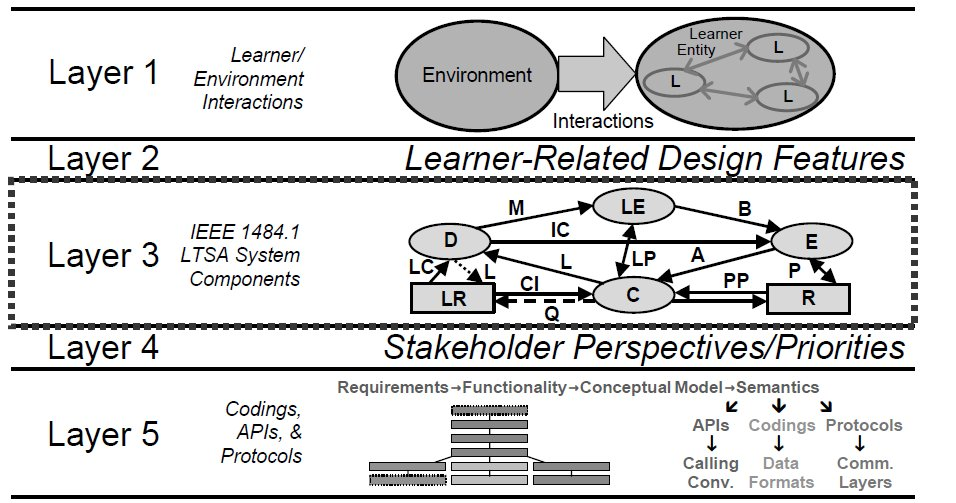
\includegraphics[scale=.4]{m.jpg}
 % m.jpg: 956x503 pixel, 72dpi, 33.73x17.74 cm, bb=0 0 956 503
 \caption{IEEE LTSA Layered Structure\cite{ltsa}}
\end{figure}
\end{comment}
\subsection{A detailed description of LTSA system components at level 3}
 \blindtext types used are \cite{ltsa} (figure.2):
\begin{enumerate}
 \item \textit{The interaction context:} This flow of data gives the necessary information for
    interpretation of the observations.
\item \textit{The observations:} This represents the real-time unabridged information concerning the learner activities.
\item \textit{The acquisition state:} The evaluating process can send or update a learner profile (e.g. a response to a correct answer within a given time).
\item \textit{The learner profile:} The tutoring process can consult and modify learner information during the apprenticeship. This is a data-store
    which updates the learner profile as per data-base management system dictat.
\item \textit{The evaluation:} It informs the tutoring process of the present state of the
    learner profile so as to optimize the learning process.
\begin{comment}
\begin{figure}[htb]
 \centering
 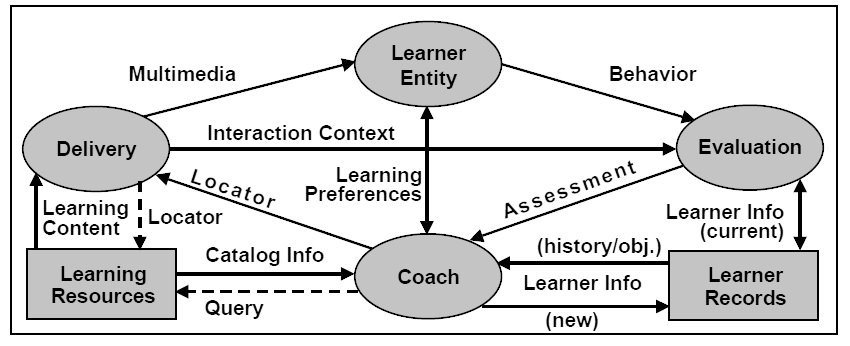
\includegraphics[scale=.6]{rj.jpg}
 % rj.jpg: 850x346 pixel, 72dpi, 29.99x12.21 cm, bb=0 0 850 346
 \caption{IEEE LTSA Layer-3 (System Components)\cite{ltsa}}
\end{figure}
\end{comment}
\item  \textit{The learner preferences:} The tutoring process negotiates the teaching parameters with the learning actor(s).
\item  \textit{The multimedia data:} This flow of data allows the learning process to use simultaneous pedagogical multimedia resources such as video, audio, text and
    graphics. All these contents are devloped and designed as per scheme of e-Learning.
\item  \textit{The locality:} This data or control flow indicates where to find a given pedagogical resource.
\item  \textit{The pedagogical contents:} This data flow has the coded pedagogical material. The content presentation, in an appropriate format, is an
    outcome of this data flow.
\item  \textit{The catalogued inquiries and information:} The tutoring process can carry out
    simple requests to find appropriate learning objects for a course. These requests
    may contain search criteria based on the learner’s preferences, the evaluation
    results and the course information.

\end{enumerate}
   The role and the behavior of the different components are described using a
learner scenario, which is divided into eight identified scenarios:
\begin{enumerate}
 \item The teaching style, the pedagogical choices and the acquisition methods are
negotiated with the learner.
\item The learning process is observed and evaluated in a context of action and
interaction with the system.
\item The evaluating process gives observations and indications about the learner
style and/or information about the functioning /the state of the system.
\item This data is stored in a data bank dedicated to the learner.
\item The tutoring process analyses the learner’s performance from his assessments,
his preferences, his past history and his future perspectives.
\item This same process searches for suitable learning object using resource bank
requests.
\item The tutoring process extracts the pedagogical content from the proposed
resources. It transmits the resource references to the diffusion process, organizing
them, for example, into a pedagogical sequence.
\item The diffusion process extracts the pedagogical contents from the learning
object to adapt it to the surrounding interface used by the learner.

\end{enumerate}

\subsection{Limitations of LTSA for e-Learning services}
Some of the functional areas, that is not included in LTSA, are identified :
\begin{itemize}
 \item The model does not regard the learning object designer as an integrated
component in the learning process.
 \item The students evaluation records are stored but, the use is not specified. This
brings ambiguity in case of e-Learning services to be provided and e-Learning services to be received to give services. 
The composition of services becomes difficult.
 \item For a distance mode learner, if the learner possesses some wrong/incomplete
idea at the start and the feedback system fails to identify it, then the LTSA layer
2 algorithm falls apart under a never ending iterative cycle. The learner can never
be sure, that his learning activities are properly registered. Moreover, the system
never recognizes the incomplete feedback or shows the partial data that may have
been registered for the future use.
 \item Students counseling is not included in the LTSA architecture. Students enrol
courses by only knowing the name of the course without knowing the prerequisites
or eligibility. Being in different service mode, these components are scheduled to
run with one another and most of the time behaves like stand-alone service module.
The selection of the courses is left to student’s rationale and intuition without a
suggestion from the mentor. The lack of student counselling makes the e-Learning
system weaker than a formal education system.
 \item The model is based on client server, component based system. There is
still possibility of making LTSA component more reuseable, loosely coupled and
increasing the modularity of LTSA by extending it into SOA environment. The
component may be used as services. But mapping the components into services
does not fit into typical Client-Server architecture.

 
\end{itemize}




\section{Mapping IEEE LTSA Framework in Client Server Model}
 \blindtext
\begin{figure}[htb]
 \centering
 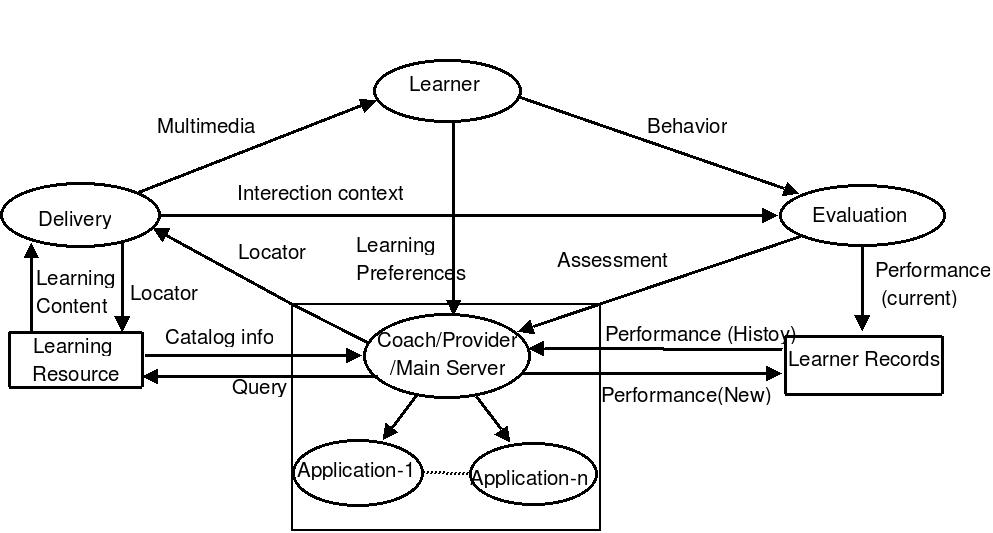
\includegraphics[scale=.5]{IeeeLtsa.jpeg}
 % IeeeLtsa.jpeg: 993x533 pixel, 72dpi, 35.03x18.80 cm, bb=0 0 993 533
 \caption{IEEE LTSA Client Server Architecture\cite{ltsa}}
\end{figure}

\subsection{Limitation of client-server based IEEE LTSA framework}
IEEE LTSA client server architecture is suitable for utilizing stand alone service
components as evident from figure. 3 These service components do not own any responsibility towards offering themselves for preparation of composite services. It is
obvious that composition compatability of services only comes as an after thought
in this architecture making it as a ’limited service’ architecture. Other limitations
are:
\begin{itemize}
 \item  Learning content provider (server) may not be able to resolve concurrency.
Many learner might try to connect to server at the same time. As any learner may
like to connect at any time, it creates a bottleneck due to lack of concurrency. Even
it may lead to typical denial of services (DoS).
 \item Since the learner and provider component may be devloped by different vendors, they may not be compatible with respect to data type, language, platform
etc.
 \item Replication of provider due to different customization may make data inconsistant.
 \item It is incapable of providing real time services and therefore, works in a limited
way in interactive mode. The security remains limited to authentication of the
learner. Multilevel security is usually not employed. The architecture generally
works in trust based security mode. It heavily relies on operating system security
features e.g. in unix OS, frequent use of 'chmod' command.
\end{itemize}
\section{Security Framework}
 \blindtext C\&C module \cite{cc}.

\section{Mapping IEEE LTSA Framework in Proposed Distributed System Architecture For Improvement}
In a distributed system, learner actively issue requests to objects in servers. Servers
passively provide access to objects that respond to client requests. Clients and
servers are usually at different address spaces. Clients and servers both may be
located on several machines physically (Figure.4). 
\begin{figure}[h!]
 \centering
 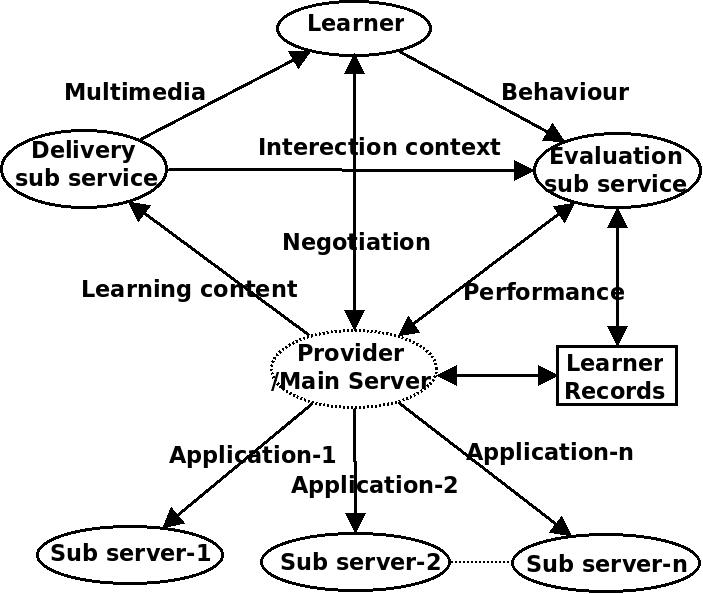
\includegraphics[scale=.5]{ds2.jpeg}
 % ds2.jpg: 961x831 pixel, 100dpi, 24.41x21.11 cm, bb=0 0 692 598
 \caption{IEEE LTSA in Distributed System Architecture}
\end{figure}

\subsection{Capabilities in the DSA for e-Learning}
Distributed system broadens the scope of service composition by implementing
compatability of services. Other capabilities of the system for e-Learning framework
are as follows:
\begin{itemize}
 \item This open system architecture allows new learning resources to be added to
it, as and when required.
 \item System is flexible and scalable.
 \item It is possible to reconfigure the system dynamically.
  \item No need to decide on locations for learning applications, each application can
work at any location.
 \item No need of providing service compatibility separately, if a standard is followed.
\item Concurrency of proccesses can be ensured by the very design of the architecutre.

\end{itemize}



\subsection{Limitation of the Architecture}
\begin{itemize}
 \item Systems are very complicated to design and implement.
\item Incapable of providing composite services unless predefined through a standard
 technology.
\item System is not as much scalable as it should be in case of e-Learning requirement
 to cater the need of different learners of different capabilities and requirements.

\end{itemize}

\subsection{Security for the proposed Distributed e-learning System}
Security remains to be closely linked with performance of a e-Learning system in
a distributed environment. While considering security from LTSA point of view,
the design elements must take care of information access control, various security
handlers and other security related processing (e.g. Kerboros or any other third
party authentication server) \cite{fox}.
\subsubsection{Information Access and Control}  \blindtext
 \subsubsection{ Security Handlers/ Processing} \blindtext
minimally considered and must be the focus of active research for preparing secured
service composition in e-Learning system \cite{car}.

\subsection{Security Challenges for the extending e-Learning services}
 \blindtext  as \cite{car}:
\begin{itemize}
 \item  \blindtext
 \item Network attacks usually target specific applications. The adaptation of control and coordination among the different mechanisms, whose capabilities are used
in the adaptive response, is needed.
\end{itemize}
 \blindtext
